\mode*
\section[Metodolog\'ia]{Metodolog\'ia}
\label{sec:metodo}

\mode<presentation>{
  \begin{frame}
    \transduration{1}
    \frametitle{C\'omo se va a resolver?}
    \framesubtitle{Hacia un framework de rob\'otica b\'ipeda}
    \begin{center}
      \LARGE \textbf{\textcolor{blueun}{Metodolog\'ia}}
    \end{center}      
  \end{frame}
  \begin{frame}
    \transduration<1->{1}
    \frametitle{C\'omo se va a resolver?}
    \framesubtitle{Hacia un framework de rob\'otica b\'ipeda}
    \begin{center}
      \only<1>{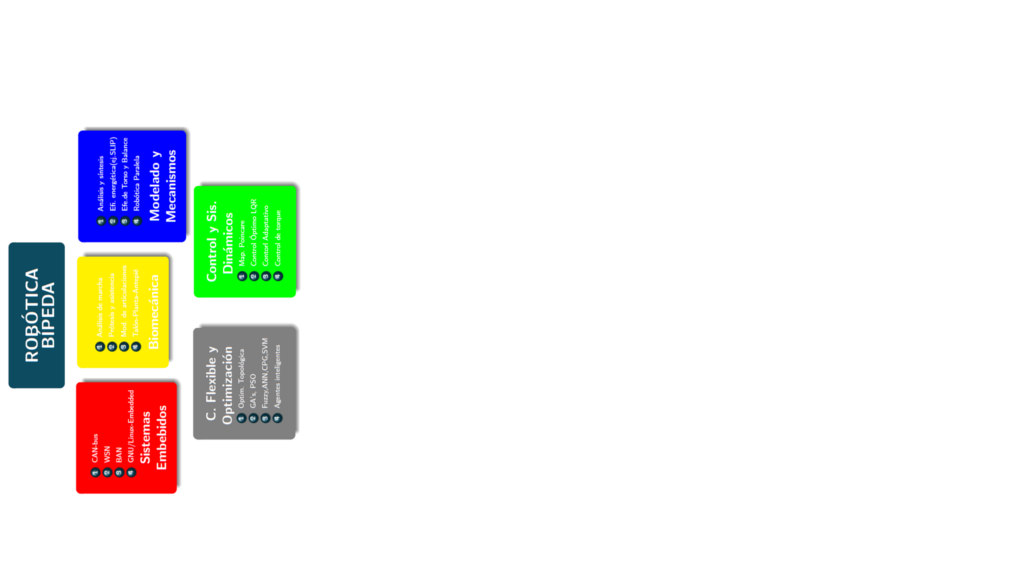
\includegraphics[width=10.5cm]{../images/MakeTheFramework_0.png}}
      \only<2>{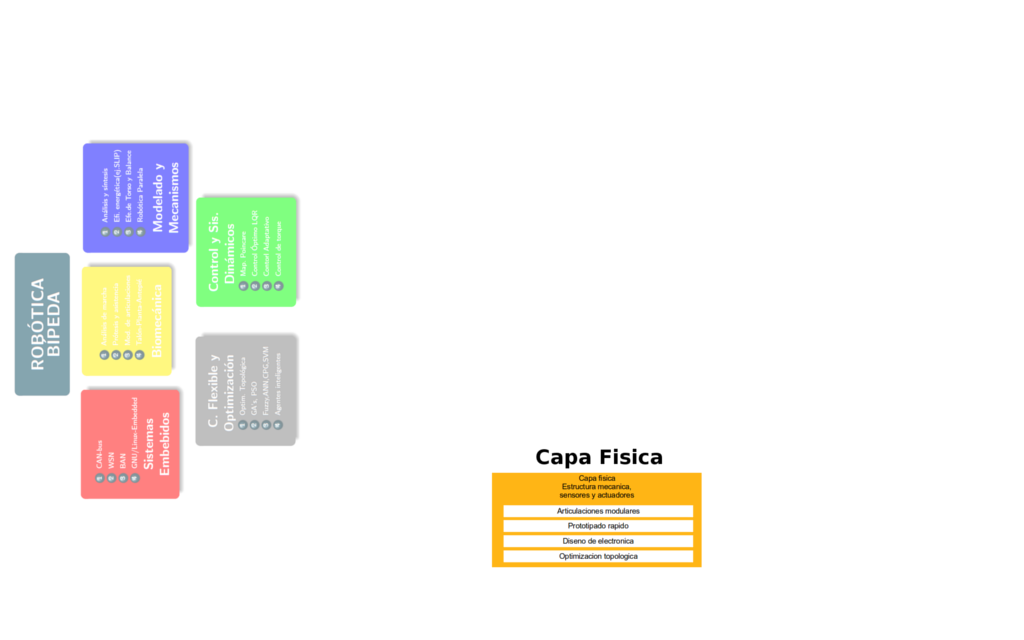
\includegraphics[width=10.5cm]{../images/MakeTheFramework_1.png}}
      \only<3>{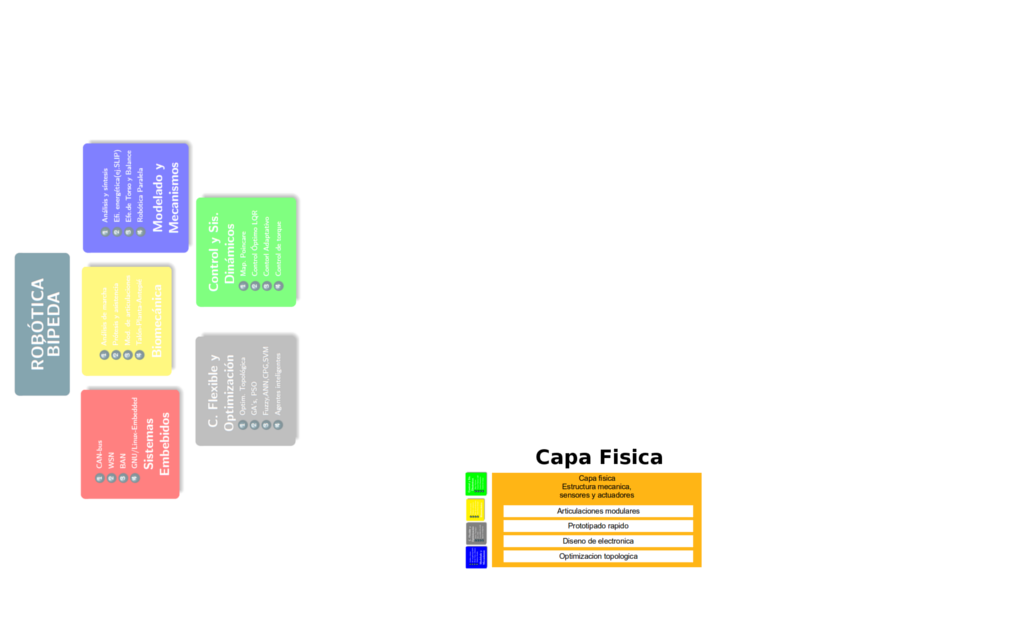
\includegraphics[width=10.5cm]{../images/MakeTheFramework_2.png}}
      \only<4>{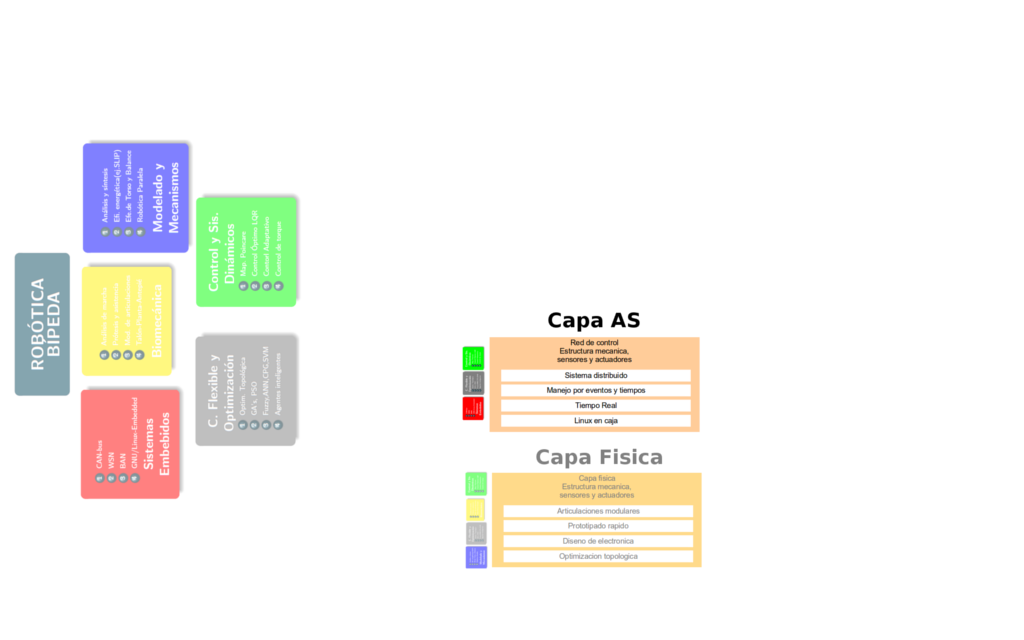
\includegraphics[width=10.5cm]{../images/MakeTheFramework_3.png}}
      \only<5>{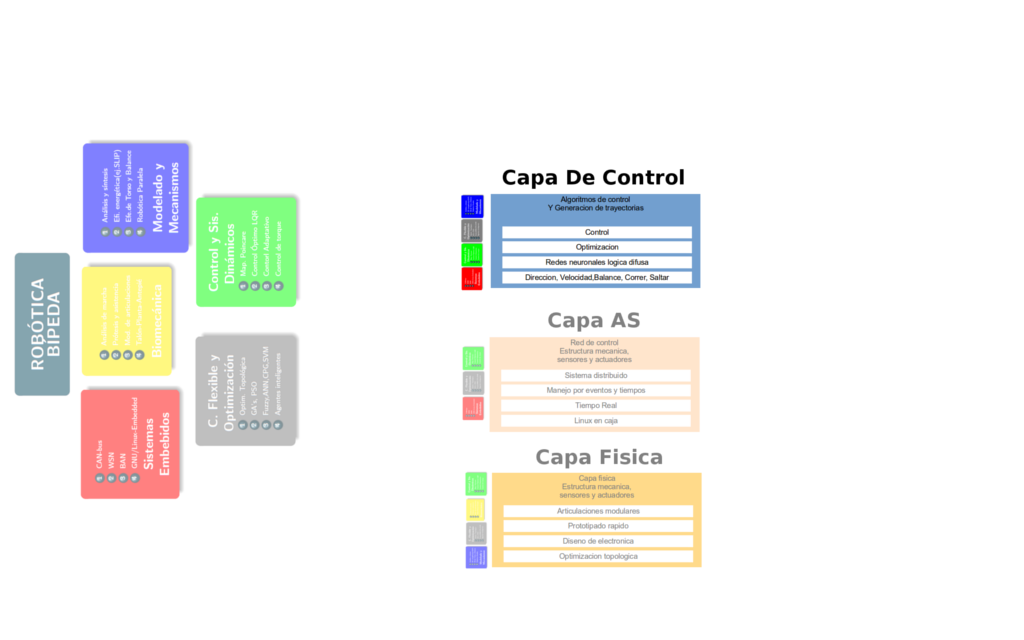
\includegraphics[width=10.5cm]{../images/MakeTheFramework_4.png}}
      \only<6>{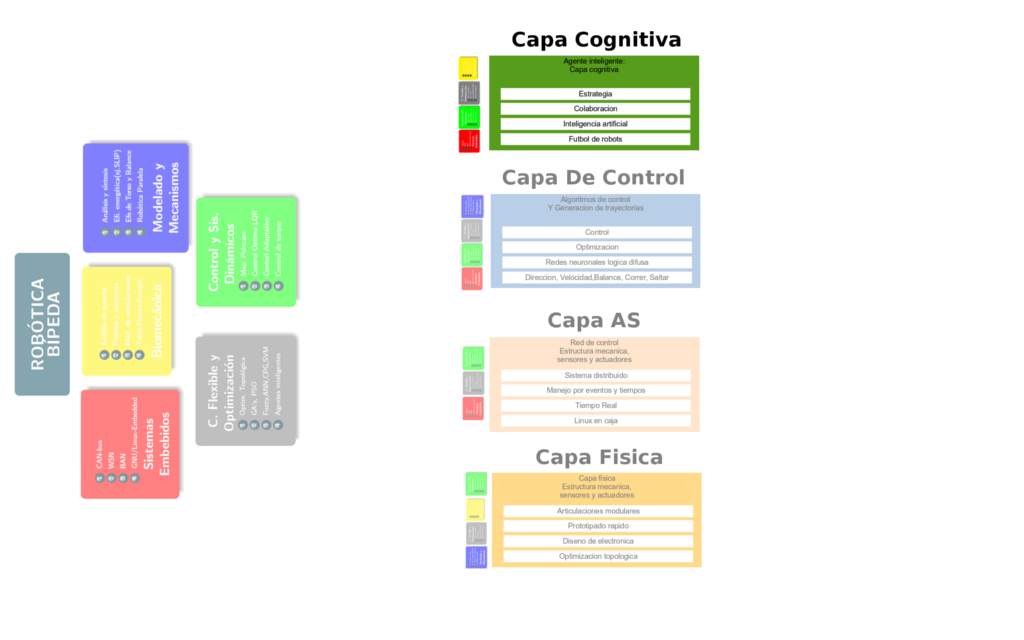
\includegraphics[width=10.5cm]{../images/MakeTheFramework_5.png}}
      \only<7>{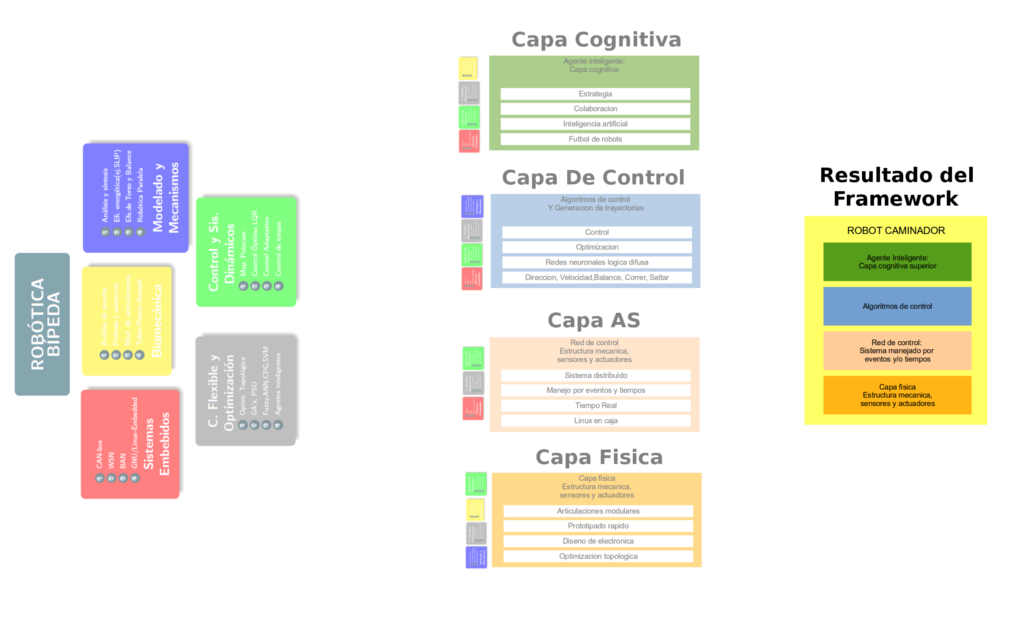
\includegraphics[width=10.5cm]{../images/MakeTheFramework_6.png}}
      \only<8>{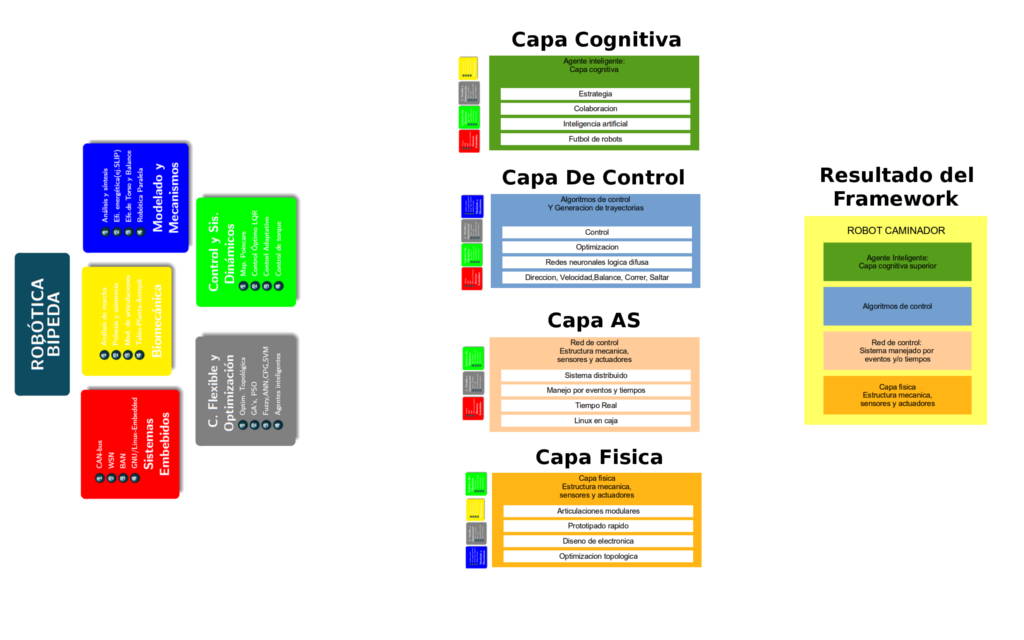
\includegraphics[width=10.5cm]{../images/MakeTheFramework_7.png}}
    \end{center}
  \end{frame}
  \begin{frame}
    \transduration{10}
    \frametitle{Como se realizar\'a esta investigaci\'on?}
    \framesubtitle{Mecanismos para su seguimiento, control y avance}
    \begin{center}
      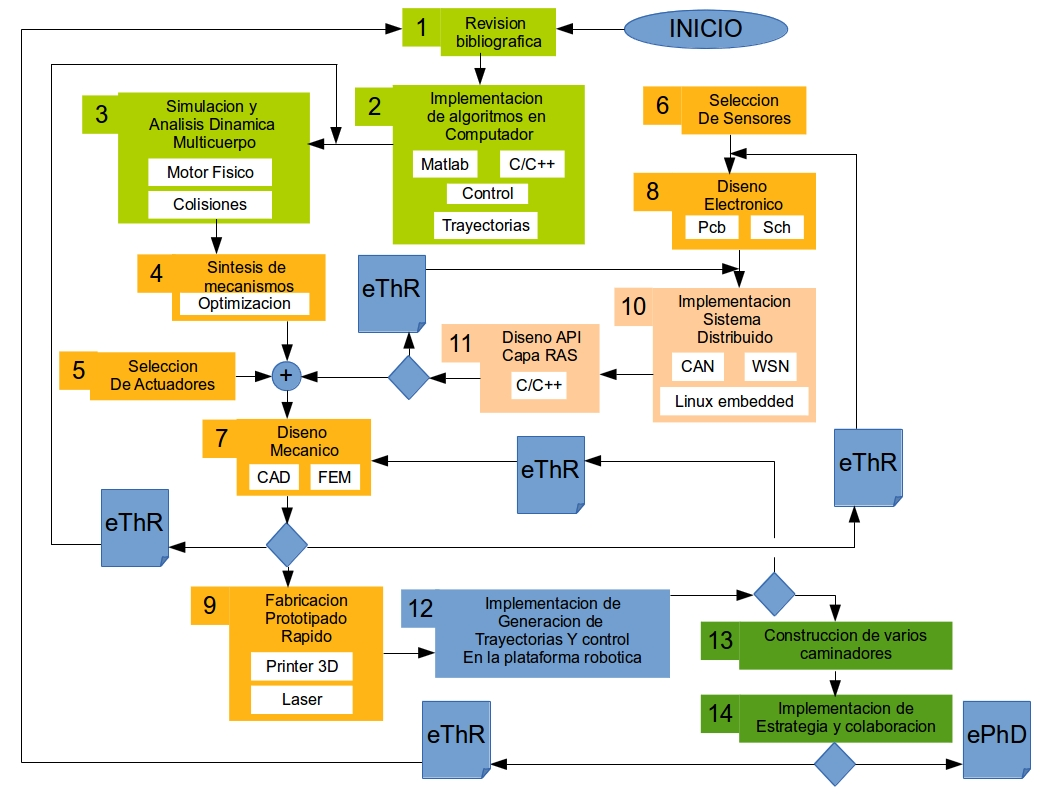
\includegraphics[scale=0.25]{../images/metGen2.png}
    \end{center}
  \end{frame}
}
El siguiente proceso se implementar\'a como mecanismo de control y realimentación de la evoluci\'on de la investigaci\'on y el adecuado avance hacia sus objetivos, se repetir\'a a lo largo del desarrollo de la tesis, el cual se iterar\'a durante al menos cinco veces, (ver Fig.\ref{fig:method}, en donde se enumeran cada uno de los pasos).
\begin{figure}[!htb]
  \centering
  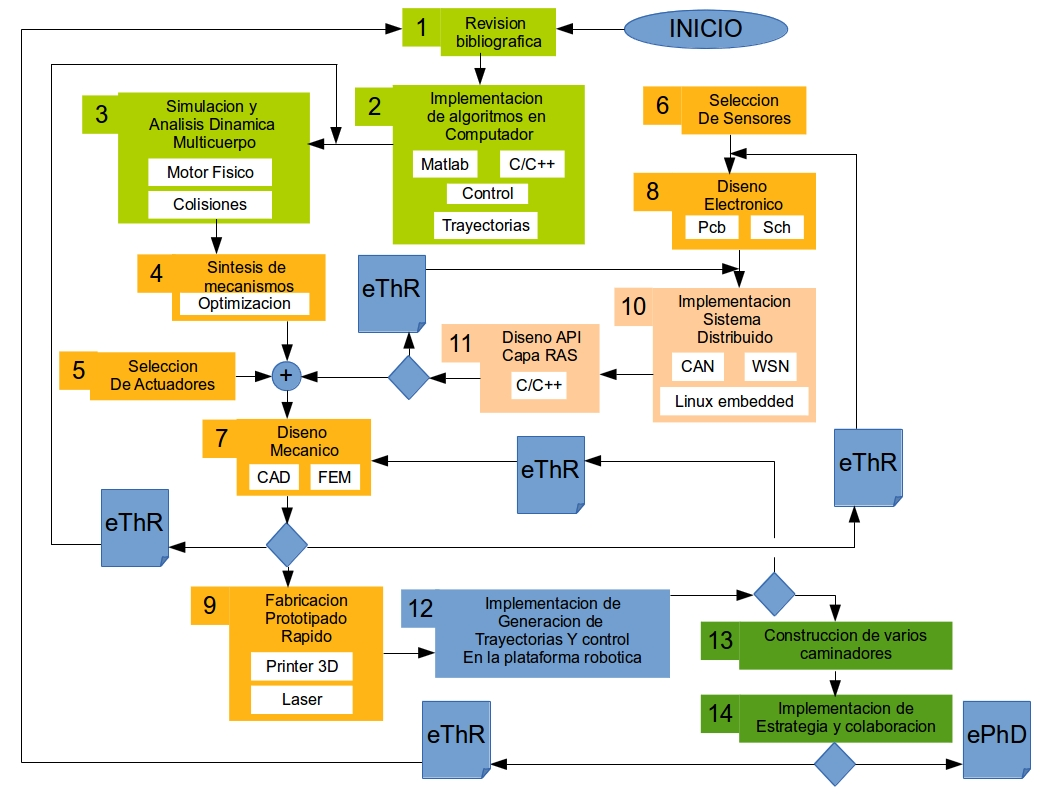
\includegraphics[scale=0.42]{../images/metGen2.png}
  \caption{Metodolog\'ia general}
  \label{fig:method}
\end{figure}
\begin{enumerate}[\textbf{Paso} 1:]
\item \textbf{Revisi\'on bibliogr\'afica -} Generar y ampliar continuamente un estado del arte sobre los temas relacionados, esto es consultar constantemente art\'iculos de revistas que se encuentren actu\'almente investigando sobre el tema. La constante actualizaci\'on del estado del arte serviar\'a para estar al tanto de nuevos avances en el tema. Continuar al \emph{paso 2}.\par
\item \textbf{Implementaci\'on computacional de algoritmos -} Se intentar\'a comprobar los resultados y consejos de los art\'iculos que sean m\'as relevantes para lograr los objetivos de la tesis. La implementaci\'on de algoritmos de control, generaci\'on de trayectoria y optimizaci\'on se realizar\'an utilizando una combinaci\'on de los lenguajes C/C++, Matlab, librer\'ias y toolboxes disponibles. En este paso es importante la seleci\'on, la generaci\'on y/o manejo de librer\'ias de mec\'anica multicuerpo. Librer\'ias como Cocos2d, Box2d, OGRE o Unity3d de uso libre y/o comercial, requieren ser analizadas en esta etapa. Continuar al \emph{paso 3}.\par
\item \textbf{Simulaci\'on y an\'alisis de la din\'amica multicuerpo - } Escogido un Framework para trabajar las necesidades requeridas para la implementaci\'on del paso 2, este paso tiene como objetivo analizar propuestas de dise\~no m\'ecanico, sugeridas por los pasos o iteraciones anteriores y probar los desempe\~nos de los algoritmos. En resumen modelar, simular, analizar y s\'intetizar mecanismos subactuados que optimicen la energ\'ia para la locomoci\'on de caminar, saltar o correr. Continuar al \emph{paso 4}.\par
\item \textbf{S\'intesis de mecanismos - } Utilizando t\'ecnicas bio-inspiradas, optimizaci\'on y algoritmos evolutivos, se har\'a una b\'usqueda de los parámetro de dise\~no que formar\'an las cadenas cinem\'aticas que propondrán una configuraci\'on b\'ipeda. Esta búsqueda optimizara el consumo de energ\'ia y tendrá en cuenta la forma de los actuadores. Continuar al \emph{paso 7}.\par
\item \textbf{Selecci\'on de actuadores - } Se deber\'a probar con distintos tipos de actuadores, motores de paso, servos, motores DC brushless, etc., que modificar\'an partes del dise\~no mecanico, en forma y en material. Etapas de potencia. Continuar al \emph{paso 7}.\par
\item \textbf{Selecci\'on de sensores - } Selecci\'on y prueba de IMUs, strain-gauges, reflectores de fuerza, sensores de temperatura, encoders, etc. Continuar al \emph{paso 8}.\par
\item \textbf{Dise\~no Mec\'anico - } El resultado de esta etapa debe ser un dise\~no robusto y en detalle de una plataforma modular capaz de configurar cadenas cinem\'aticas controladas y/o monitorizadas bajo el sistema distribuido. Adem\'as los disen\~os ser\'an basados en la caminata pasiva y el almacenamiento de energ\'ia mediante elementos pasivos que dejan como resultado los pasos anteriores. Si el dise\~no no es fabricable y el hilo de iteraci\'on es mec\'anico ir al \emph{paso 3} y escribir un reporte t\'ecnico, preparaci\'on para ponencias o congresos. Pero si el dise\~no no es fabricable y el hilo de iteraci\'on es electr\'onico ir al \emph{paso 8} si es fabricable ir al \emph{paso 9} y escribir un reporte t\'ecnico, preparaci\'on para ponencias o congresos.\par
\item \textbf{Dise\~no Electr\'onico - } Dise\~no de esquemas electrónicos, selección de ICs y fabricaci\'on de tarjetas (PCBs), para pruebas del sistema de la capa RAS. Continuar al \emph{paso 10}.\par
\item \textbf{Fabricaci\'on prototipo r\'apido - } Se construir\'a una plataforma rob\'otica modular y fabricada por prototipado, impresión 3D o corte por láser (ver Figura \ref{fig:objCapas} Capa Física). Continuar al \emph{paso 12}.\par
\item \textbf{Implementaci\'on del Sistema Distribuido - } Fabricaci\'on de PCBs de prototipo o definitivas, y pruebas sobre la red. Pruebas y manejo de CANbus, ZigBee y BLE. Definición de las tramas de comunicaci\'on. Continuar al \emph{paso 11}.\par
\item \textbf{Dise\~no API Capa RAS - } Implementar librerías en C/C++ que permita organizar la red de sensores y actuadores para que funciones en tiempo real organizando los procesos del sistema para que sean manejados por eventos o por temporizaci\'on por un controlador central con Linux embebido. Si se logra el requisito de tiempo-real continuar al \emph{paso 7}, si no ir al \emph{paso 10} y escribir un reporte t\'ecnico, preparaci\'on para ponencias o congresos.\par
\item \textbf{Implementación en la Plataforma Rob\'otica - } En esta etapa se prueban sobre la plataforma rob\'otica los algoritmos implementados en el computador en los pasos anteriores. Si el desempe\~no es el adecuado continuar al \emph{paso 13}, si no regresar a la etapa de dise\~no en el \emph{paso 7} y escribir un reporte t\'ecnico, preparaci\'on para ponencias o congresos.\par
\item \textbf{Construcción de varios prototipos - } Esta etapa despu\'es de probar que la plataforma construida funciona adecuadamente como agente individual, se construir\'an m\'as plataformas para que pueda interactuar entran a estudiar los agentes inteligentes en grupo. . Continuar al \emph{paso 14}.\par
\item \textbf{Implementaci\'on Agente Inteligente - } Aceptado un prototipo funcional de la plataforma hasta la capa de control se deberá  implementar estrategias y actividades colaborativas usando una red de caminadores  (ver Figura \ref{fig:objCapas} Capa Cognitiva.). Si se logra todos los objetivos finalizar escribiendo el documento final de la tesis, si no ir al \emph{paso 1} escribiendo un reporte t\'ecnico general de la iteraci\'on investigativa, preparaci\'on para ponencias o congresos.\par
\end{enumerate}
El tiempo que se tome en cada uno de los pasos anteriores ser\'a seg\'un se necesite, aunque inicialmente se dar\'a un tiempo limite seg\'un el cronograma del proyecto.\par

